\documentclass[10pt]{article}

\usepackage[left=.5in, right=.5in, top=.3in, bottom=.5in]{geometry}
\usepackage{amsfonts,amsmath,amssymb}
\usepackage{authblk}
% \usepackage{hyperref}
%% put affiliations into one line
\makeatletter
\renewcommand\AB@affilsepx{\quad\protect\Affilfont}
\usepackage{bbm}
\usepackage[inline]{enumitem}
\usepackage{graphicx}
\graphicspath{{./}{../image/}}
\usepackage[colorlinks=true,citecolor=blue,urlcolor=blue]{hyperref}
\usepackage{natbib}
\usepackage{setspace}
\setstretch{1.2}
\usepackage{titlesec}
\titlespacing*{\section}{0pt}{5pt}{5pt}

\newcommand{\EE}{{\mathbb{E}}}
\newcommand{\PP}{{\mathbb{P}}}
\newcommand{\QQ}{{\mathbb{Q}}}
\newcommand{\Fb}{\mathbf{F}}
\newcommand{\Ib}{\mathbf{I}}
\newcommand{\hb}{\mathbf{h}}
\newcommand{\xb}{\mathbf{x}}
\newcommand{\one}{\mathbbm{1}}
\newcommand{\Ocal}{\mathcal{O}}


\begin{document}


\title{\vspace{-1cm} \Large
Progress Report: Transformer-CRF Integration for Sequence Labeling on EEG Data}

\author[1]{Xiaohang Ma}
\author[2]{Shiying Xiao}
\author[2]{Xiaohui Yin}

\affil[1]{Department of Mathematics, UConn}
\affil[2]{Department of Statistics, UConn}

\date{\vspace{-1.3cm}}

\maketitle


\section{Progress}
% Overview of progress made and key accomplishments.


The project is progressing according to schedule. To date, we have made
significant strides in several key areas:
\begin{enumerate}
\item Model Development:
We have initiated development of a convolutional neural network (CNN) combined
with a hidden conditional random field (HCRF). This hybrid approach aims to
create a robust image segmentation framework capable of capturing both local
and global dependencies within the data structure.
\item Variational Inference Implementation:
To efficiently approximate the posterior distributions in our complex model,
we have integrated variational inference into the HCRF component.
This technique is particularly effective in handling the computational
challenges posed by the dataset's heterogeneity.
\item Data Preprocessing:
% We have finished data preprocessing of the eeg figures and spectrogram image. We transformer the 
% eeg signals to spectrograms through build-in functions from open source libraries like OpenCV and PyWavelets.
% We then concate these spectrograms as a \(512 \times 512\) image, which is ready to be feeded in our model.
We completed the data preprocessing for EEG signals and their corresponding spectrograms. The EEG signals were transformed into spectrogram images using built-in functions from open-source libraries such as OpenCV and PyWavelets. We then concatenated these spectrograms into a \(512 \times 512\) image, which is now ready for input into our model.
\end{enumerate}
%This progress has provided a foundation for the next
%steps of our research.


\section{Preliminary Results}
% Summary of initial findings and analyses.

In our model, the variable \(y \) represents the corresponding brain signal label of the inpute image \(\mathbf{x}\). 
The hidden variable \(\mathbf{h} = \{h_{i}\}\) represents the label at each pixels of \(\mathbf{x}\). The parameter \(\theta\)
contain parameters of neural networks as well as the HCRF.
We introduce the potential functions of our HCRF model as:
\begin{equation*}
\Phi(y, \hb, \xb; \theta) = \underbrace{
\sum_{j \in \nu} \phi(h_j, x_j; \omega) +
\sum_{i \neq j} \psi(h_i, h_j, x_i, x_j; \eta)}_{
% \propto \log\PP( \hb \vert \xb; \theta)
\textrm{Measures log-likelihood $\log\PP(\hb \vert \xb; \theta)$}}
+ \underbrace{
\sum_{j \in \nu} \varphi(y, h_j, x_j; \delta) + \vartheta(y, \xb; \varpi)
}_{
% \propto \log\PP(y | \hb, \xb; \theta)
\textrm{Measures log-likelihood $\log\PP(y \vert \hb, \xb; \theta)$}
}
\end{equation*}


\begin{itemize}
\item \textbf{Unary Potential}
$\phi(h_j, x_j; \omega)$ measures the likelihood of the local feature
$x_j$ is assigned as the hidden attention state $h_j$.
We generate the likelihood through a softmax operation on $\Fb(\xb)$
the feature maps of CNN with $(N, C_{\textrm{out}})$ dimensions,
by which the potential of each pixel $x_j$ assigned as each state of
hidden state set $\{0, 1, \dots, 5\}$
is drawn and represented by a matrix with $(N, 2)$ dimension.
\item The parameter $\varpi$ will be learned by end-to-end CNN-Unet
training structure.
\item \textbf{Unary Potential} $\varphi(y, h_j; \delta)$ measures
the compatibility between global class label $y$ and the hidden local
state $h_j$. This potential is parametrized as:
\begin{align*}
\varphi(y, h_{j}; \delta) = \sum_{a \in Y} \sum_{b \in H} \delta_{a, b}
\cdot \one(y = a) \cdot \one(h_j = b).
\end{align*}
\item \textbf{Binary Potential} $\psi(h_i, h_j, x_i, x_j; \eta)$
balances the hidden label compatibility of the neighboring pixels on the 
feature image $\Fb(\Ib)$.
We define this potential through a common contrast-sensitive two-kernal 
potentials~\citep{krahenbuhl2011efficient,chen2022end}:
\begin{equation*}
\psi(h_i, h_j, x_i, x_j; \eta) = \mu(h_i, h_j) \Bigg[
\omega_1 \exp \left(
-\frac{\left\lvert p_i - p_j \right\rvert^2}{2\eta_\alpha^2}
-\frac{\left\lvert \Fb_i(\Ib) - \Fb_j(\Ib) \right\rvert^2}{2\eta_\beta^2} 
\right) + \omega_2 \exp \left(
- \frac{\left\lvert p_i - p_j \right\rvert^2}{2 \eta_\gamma^2}
\right)
\Bigg]
\end{equation*}
\end{itemize}


The mean-field varepsilon family approximation of
$\log\PP(\hb \vert y, \xb; \theta)$ as $\QQ(\hb) = \prod_{i=1}^N q_i(h_i)$.
Then the evidence lower bound under the mean-field family is given by
\begin{equation*}
\begin{split}
& \textrm{ELBO}(\QQ) = \EE_{\QQ(\hb)} \log\PP(y, \hb \vert \xb; \theta)
- \EE_{\QQ(\hb)} \log q(\hb) = \sum_{i=1}^N \EE_{q_i(h_i)}
\left[ \phi(h_j, x_j; \omega) + \varphi(y, h_j, x_j; \delta) \right]
+ \sum_{i=1}^N \sum_{j=1}^N \sum_{l,l^\prime} \one_{\{i \neq j\}}\QQ(h_i = l) \\
&\quad \QQ(h_j = l^\prime) \mu(l, l^\prime)
\Bigg[ \omega_1 \exp \left(
- \frac{\left\lvert p_i - p_j \right\rvert^2}{2\eta_\alpha^2}
- \frac{\left\lvert \Fb_i(\Ib) - \Fb_j(\Ib) \right\rvert^2}{2\eta_\beta^2}
\right)
+ \omega_2 \exp \left(
- \frac{\left\lvert p_i - p_j \right\rvert^2}{2\eta_\gamma^2}
\right) \Bigg]
- \sum_{i=1}^N \EE_{q_i} \log q_i(h_i) + \vartheta(y, \xb; \varpi).
\end{split}
\end{equation*}


By the coordinate ascent variational inference(CAVI) algorithm,
we can obtain that fix $q_j(h_j), \forall j \neq i$, the optimal $q_i(h_i)$
that maximizes $\textrm{ELBO}(q_i(h_i))$ is given by
$\QQ(h_i) \propto \exp\{\EE_{\QQ(\hb_{-i})}
\log\PP(y, h_i, \hb_{-i} \vert \xb; \theta)\}$.
Thus, we can get that
\begin{equation*}
\begin{aligned}
& q_i(l) = \\
&\frac{1}{Z_i} \exp \left\{
\phi(h_j, x_j; \omega) + \varphi(y, h_j, x_j; \delta)
+ \sum_{j \neq i} \sum_{l^\prime} q(l^\prime) \mu(l, l^\prime) 
\left[ \omega_1 \exp \left(
- \frac{\left\lvert p_i - p_j \right\rvert^2}{2\eta_\alpha^2}
- \frac{\left\lvert \Fb_i(\Ib) - \Fb_j(\Ib) \right\rvert^2}{2\eta_\beta^2}
\right)
+ \omega_2 \exp \left(
- \frac{\left\lvert p_i - p_j 
\right\rvert^2}{2\eta_\gamma^2}
\right)
\right]
\right\}
\end{aligned}
\end{equation*}


% While the models are still under development and optimization,
% initial results are promising. 
% For instance, Figure~\ref{fig:SEIZURE_3}
% illustrates a sample prediction with ground truth 94.\% Seizure and 2.9\% LPD.
% Our model predicts 88.4\% Seizure and 1.6\% LPD.
% Yellow highlights indicate the regions where the model focused its attention.
% These preliminary results show trends that are consistent with our initial
% hypotheses. The visualizations have proven useful in pinpointing areas for
% further investigation, and 
% The derived formulas appear to be robust and
% aligned with the expected model outcomes. Further analysis will refine
% these findings and explore additional dimensions of data.
After building the theoretical model formualtion of our project, we also finished 
 preliminary analyses of the data.
Our preprocessed spectrograms dataset that are ready for training model.
The dataset are available:{https://github.com/Carol-seven/Transformer-CRF\_EEG/tree/main}.

% \begin{figure}[tbp]
% \centering
% % 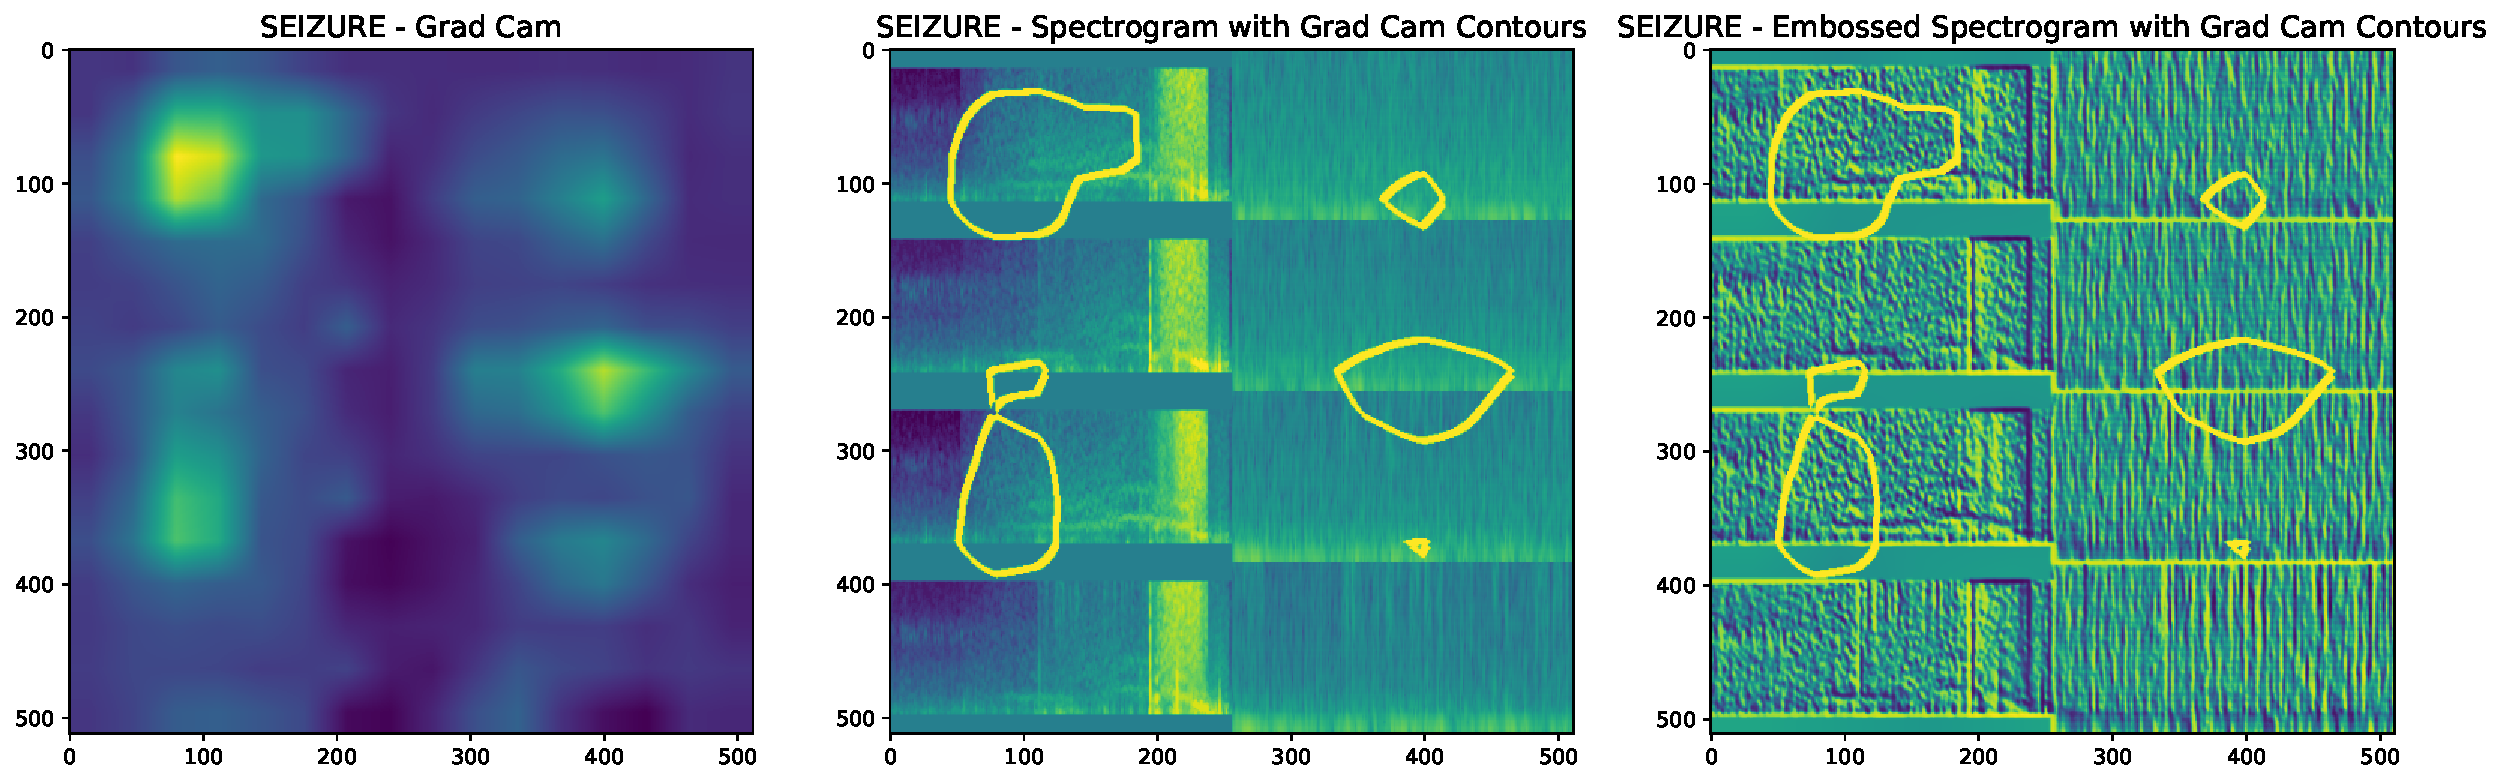
\includegraphics[width=.7\textwidth]{grad_cam_SEIZURE_3}
% \caption{An example of data visualization. Areas highlighted in yellow
% indicate regions where the model focused its attention during this specific
% prediction.}
% \label{fig:SEIZURE_3}
% \end{figure}


\section{Challenges}
% Discussion of any challenges faced during the project.


We encountered minor challenges related to data handling and computational
limitations. In particular, the complexity of certain calculations required
additional processing time, which slightly delayed our progress.
We are currently exploring ways to optimize these computations.


\section{Plan Changes}
% Outline of any adjustments made to the original plan.
% At this stage, 
% \noindent
% \textcolor{blue}{
	% Based on extra literature reviews and our preliminary results, we have made two major adjustments to our project.
	\begin{itemize}
		\item \textbf{CRF Layer Modification:} Our motivation for introducing the CRF layer was to allow the model to identify regions of input 
		images that correspond to abnormal brain activity signals. However, the original dataset, including spectrograms 
		and EEG-transformed spectrograms, lacked segmentation information, so no labels were available to train the CRF. 
		Our initial solution was to generate pixel-wise CRF labels based on the global ground truth distribution. 
		However, further review revealed that this approach could lead to isolated label regions, counteracting 
		our intent for CRF integration. Consequently, we modified the CRF layer to a hidden CRF (HCRF) 
		by setting pixel labels as hidden variables and adopted a variational inference framework to manage
		 these hidden variables in the CRF model.
		\item \textbf{Model Structure Adjustment:}We replaced the Transformer-based architecture with a U-Net CNN structure. This choice reflects 
		findings in recent research that fine-tuning large models like Transformers can be time-consuming. Instead,
		 we opted for the well-established U-Net CNN, a classical model for image segmentation, 
		 which integrates effectively with the CRF layer.
	\end{itemize}
% }
% we have not made significant changes to our original plan.
% However, due to the complexity of the dataset and model, we may consider
% slightly adjust the project timeline to allocate additional time for
% model fine-tuning.


\section{Next Steps}
% Description of remaining tasks and strategy for completion.


The remaining tasks include:
\begin{enumerate*}[label = (\roman*)]
\item Expanding and refining the visualizations based on updated data.
\item Finalizing the conduction of the neural network model including the Unet CNN layer, HCRF layer based on the formulas we have derived.
\item Training and tuning the model on our preprocessed data. 
\item Conducting a comprehensive analysis with the refined model.
\item Preparing the final report and presentation materials.
\end{enumerate*}


\section{Updates}
% Additional relevant updates or future directions.


We will provide regular updates on model performance, challenges encountered,
and any significant changes to the project plan.


\bibliography{../manuscript/refs}
\bibliographystyle{chicago}

\end{document}

%%% Local Variables:
%%% mode: latex
%%% TeX-master: t
%%% End:
